\documentclass[12pt,a4paper]{book}
\usepackage[paperwidth=14cm,paperheight=21cm]{geometry}
\usepackage{fancyhdr}
%% \usepackage{graphicx}
\setlength{\parskip}{.4cm}
\addtolength{\textwidth}{4mm}
\addtolength{\textheight}{4mm}



\title{%% \LARGE
  {\emph{The Essence of Sri Aurobindo}}}
\date{}

%% \author{Bruce Elliot}

\chead{The Essence of Sri Aurobindo}

\begin{document}

%% NOTE: Uncomment the following paragraph for the front cover
%% \thispagestyle{empty}
%% 
\includegraphics{frontCover.jpg}
%% \newpage

%% \Large
\thispagestyle{empty}
\maketitle


\
\vspace{2cm}
\begin{center}{\bf Acknowledgment}\end{center}
\thispagestyle{empty}

My acknowledgment and thanks to the Sri Aurobindo Ashram Trust for
permission to use extracts from Sri Aurobindo's magnificent works.

\vspace{1.5cm}

\begin{center}
\copyright copyright Bruce\\
email: bruce.elliot1@gmail.com\\
December, 2011\\
\vspace{1cm}
Designed \& published by\\
Prisma\\
Aurolec/Prayogashala, Auroville 605101, Tamil Nadu, India\\
email: prisma@auroville.org.in\\
\end{center}
\newpage

\pagestyle{plain}
\begin{center}\section*{Introduction}\end{center}

The Essence of Sri Aurobindo will be presented in two summaries; one
called the \emph{Bare Bones} and the other \emph{Bones With Flesh}. I
have chosen these titles so as to contrast them with the ultimate
summary, \emph{The Full Robust Body Of Truth}, which to me will only
be found in the depths of our own inner selves.

My reason for writing these is twofold: To give an outline of Sri
Aurobindo's works to those who want only the bare essentials, and to
give a deeper more comprehensive picture to those who want more, but
not too much more.

Most people I've spoken with simply find Sri Aurobindo's prose too
difficult to enjoy, and the mystic poetry of Savitri, his masterpiece,
beyond their reach. As for his prose, I feel the addition of more
commas and some parenthetical brackets would have made things easier,
but I'm quite sure some of his fluid poetic-prose style and its grand
rhythms would have been lost---that breathless speed and confidence of
a photographic memory. The English of Savitri is impeccable, but the
difficulty is in this new form of mystic poetry and its inherent depth
of spiritual knowledge. Of course anyone with even the slightest
sensitivity to spiritual poetry can peek below the surface and gain
some experience of its truth, but to get to any significant depth a
combination of patience and sincerity is needed, along with a
willingness to let its rhythm and sound pull you in.

To complete the introduction three very important things have got to
be presented:

\subsection*{First, Sri Aurobindo}

Sri Aurobindo was extraordinary in many ways and unique in his moment
of history.

\begin{itemize}
\renewcommand{\labelitemi}{$\diamond$}

\item He recorded his spiritual experiences in detail.

\item He had easy access to all the religious and spiritual
  information that came before him.

\item He had a photographic memory which helped tremendously his
  reading speed and comprehension.

\item He mastered all the classic languages including Sanskrit, and
  the poetry of these languages.

\item He was gifted with an impartial mind that could synthesize the
  most complex and contrary ideas and transcribe the result into his
  marvelous English.

\item He could read about some secret or rare experience, then go into
  a state of deep concentration (raising his consciousness to
  remarkable heights), and verify or dismiss its truth.

\item He had realized and made part of himself the three major
  spiritual experiences:

\begin{itemize}

\item Cosmic Consciousness: seeing himself in everything and
  everything in himself; thus living as his true self, the soul,
  clearly detached from the surface ego.

\item Nirvana: The passive and complete absorption into God's immobile
  silence and peace.

\item Finding that the Cosmic Consciousness and Nirvana exist together
  like two sides of one coin; both real at the same time.
\end{itemize}

\item He discovered a fourth realization; Supermind. It's one of the
  original branches of God that controls the descending and ascending
  steps of thought and mind.
\end{itemize}


\subsection*{Second, God---the basic meaning}


This is perhaps the most used and controversial word in all
languages. A word that is the foundation of all religions, and used in
general for spiritual seekers. In English, it's a simple three letter,
one syllable, soft sounding word with more power than the nuclear
bomb, and containing both benevolent and malevolent results.

The dynamics of word power will be discussed in \emph{Bones With Flesh}, but
for now our focus is on the word ``God.''

One of the greatest controversies is God representing the image of a
human being, in particular an elderly man who reasons and acts like a
human but with total power. To many people this is self-evident and
natural, but to others it's absurd and repulsive.

\noindent Sri Aurobindo explains it this way:

The word ``God'' carries infinite images, some being personal and some
impersonal, some with features and some featureless. Each soul or
person is unique, and part of that uniqueness is its relation to God,
and this relation can, and probably does, change over the course of
its evolution; most likely vacillating between pure love and decadent
hatred, between fanatical affirmation and blunt denial. But these are
all part of God's storehouse of images which he uses, lovingly, for
each soul's growth and the goal of his creation.

Sri Aurobindo has chosen to use the word ``God'' in the masculine
sense, but only because it fits smoothly into the English
language. However, for the impersonal God he uses words like the
\emph{One}, \emph{That}, the \emph{Unknowable}, etc.

Because of his infinite power, God can create whatever, wherever, and
whenever he wants; so to those who need a featured image that image
can appear, whether it be human, animal, bird or any physical shape;
it can be any race or gender. For those who desire a featureless God,
it can come as an idea, ideal, a thought or the feeling of a
Presence. Both the featured and the featureless can communicate in
whatever language or format is desired.


\subsection*{Third, Savitri}

This is Sri Aurobindo's masterpiece and foundation of all his works
and experiences.  It's a new type of mystic poetry that offers to the
reader a powerful tool for gaining access into the spiritual worlds.
It began only as an attempt to record those experiences, but not as a
poem per se. Over a period of some thirty years it grew into a poem
with over twenty four thousand lines. But its importance is in the
poetry itself. Each line developed for the perfect rhythm, word power,
tone and symbol that would allow the reader to ``feel,'' ``see'' and
``hear'' what was experienced. However, Savitri's surface drama and
philosophy is somewhat similar to the top of an iceberg, but what's
below is not at all similar. The top can increase or decrease, be
measured and weighed; the poem's depths are infinite and eternal; and
to experience these depths, the ``feeling,'' ``seeing'' and
``hearing'' will not come easily. If you read the following quotes you
should understand the difficulty:

\begin{itemize}
\renewcommand{\labelitemi}{$\diamond$}
\item ``Savitri is a record of a seeing, of an experience which is not
  of the common kind and is often very far from what the general human
  mind sees and experiences. You must not expect appreciation or
  understanding from the general public or even from the many at the
  first touch; as I have pointed out, there must be a new extension of
  consciousness and aesthesis to appreciate this new kind of mystic
  poetry.''\footnote{Sri Aurobindo, Letters on Poetry and Art: CWSA
    Vol.27, P.343}

\item ``But if I had to write for the general public, I could not have
  written Savitri at all. It is in fact for myself that I have written
  it and for those who can lend themselves to the subject-matter,
  images and technique of mystic poetry.

  ``This is the real stumbling-block of mystic poetry and especially
  mystic poetry of this kind. The mystic feels real and present, even
  ever present to his experience, intimate to his being, truths which
  to the ordinary reader are intellectual abstractions or metaphysical
  speculations. He is writing of experiences that are foreign to the
  ordinary mentality.''\footnote{Ibid, P.315}

\item ``Rapid transition from one image to another are a common
  feature in \emph{Savitri} as in most mystic poetry. In such a race
  of rapid transitions you cannot bind me down to a logical chain of
  figures or a classical monotone.''\footnote{Ibid, P.311}

\item ``You must take the idea as a whole and in all its transitions
  and not press one detail with too literal an
  insistence.''\footnote{Ibid, P.312-313}

\item ``But here several fundamental issues arise. First of all, are
  words like Inconscience and Ignorance necessarily an obstruct
  jargon? If so, do not words like consciousness, knowledge
  etc. undergo the same ban?\ldots Inconscient and the Ignorance may
  be mere empty abstractions and can be dismissed as irrelevant jargon
  if one has not come into collision with them or plunged into their
  dark and bottomless reality. But to me they are realities, concrete
  powers\ldots''\footnote{Ibid, P.314}

\item ``To the mystic there is no such thing as an
  abstraction. Everything which to the intellectual mind is abstract
  has a concreteness, substantiality which is more real than the
  sensible form of an object or of a physical event. To me, for
  instance, consciousness is the very stuff of existence and I can
  feel it everywhere enveloping and penetrating the stone as much as
  man or the animal.''\footnote{Ibid, P.316}

\item ``The poem he quotes from Blake is certainly not nonsense, but
  has no positive and exact meaning to the intellect or the surface
  mind; it expresses certain things that are true and real, not
  nonsense but a deeper sense which we feel powerfully with a greater
  stirring of some inner emotion, but any attempt at exact
  intellectual statement of them sterilizes their sense and spoils
  their appeal.''\footnote{Ibid, P.317}

\item A poet friend of Sri Aurobindo had asked him to say something
  about the white-fire dragon-bird in Savitri. Sri Aurobindo replied:
  ``All birds in that region are relatives. But this is the bird of
  eternal ananda, while the Hippogriff is the divinised thought and
  the bird of fire is the Agni-bird, psychic and tapas. All that
  however is to mentalize too much and mentalizing always takes most
  of the life out of spiritual things. That is why I say it can be
  seen but nothing said about it.''\footnote{Ibid, P.294}
\end{itemize}

If you'll note how Sri Aurobindo qualifies ``mentality'' you'll see
he's talking only about the lower and outward aspects of the mind. For
example; ``general human mind,'' ``ordinary mentality'' and ``surface
mind.''

The mind has its role in reading Savitri, but not so much its
analyzing and reasoning capacities as in its deeper capacities of
``seeing,'' ``feeling'' and ``hearing'' that hold a much greater truth
than the lower and outward mentality; and yet the lower can be
nourished on rich spiritual philosophies as it grows into the higher
ranges.

This is where the Essence comes in. To give to those people who want
or need a surface mind diagram based on Sri Aurobindo's experiences, I
offer my two summaries, but remember they are an essence, not a
complete.


\newpage
\chapter*{The Bare Bones}


As it was stated in the introduction, this short summary of Sri
Aurobindo's spiritual experiences is meant for people with a poor
English background and/or who are overwhelmed by the mass and style of
his writing. Here you are given the bare bones and streamline picture
of creation, its importance for us human beings, and its aim on Earth.

The word ``God'' is central to both summaries, and the introduction's
meaning should be read first. The repetition of ``God'' is on purpose,
and used to reinforce the supreme point that he alone is the complete
reality; and that us souls, though given a conditional independence,
are always under his blissful control, and exist only by his
stupendous power of love .

\noindent We'll now begin with the Bare Bones summary:

\begin{itemize}
\renewcommand{\labelitemi}{$\diamond$}
\item God is the only ultimate reality, and is undefinable or has
  infinite definitions.

\item Above creation God exists in a motionless state.

\item God created the universe to experience himself in action.

\item God created the universe from his own Being; he therefore
  \emph{Is} everything, is \emph{In} everything, and is more than everything,
  all at the same time.

\item God has infinite Power, Knowledge, Bliss and Love.

\item God created the soul as a unique living portion of himself that
  represents one viewpoint of his Reality.

\item God created the surface person i.e. name, ego, body, mind and
  senses(that function like a puppet or machine), so that the drama of
  life could be staged.

\item God covered each soul with Ignorance and forced it to identify
  with the surface person so that it would experience specific aspects
  of the drama that are acted out by the surface person i.e. joys,
  pains, emotions, sufferings, etc.

\item Each soul, when finished with its allotted experiences, would
  then be shown its true self.

\item Each soul would have gone through many rebirths before knowing
  its true self.

\item Each new enlightened soul would exchange its surface identity
  and personality for one that is divine, based on its past
  experiences; and would enjoy a conscious relationship with God.

\item Each new enlightened soul would have three choices:

\begin{itemize}
\item To merge back into God.
\item To keep its divine identity and personality and live in a paradise.
\item To keep its divine identity and personality and return to Earth,
  to help create the kingdom of God there; where matter will also be
  alive to the Truth.
\end{itemize}
\end{itemize}


\chapter*{Bones With Flesh}

Here you'll be presented with the mechanics and architecture of God;
an impossible feat for human intelligence, and yet even a roughly
constructed outline can be quite useful to our craving minds,
especially if its building material has come from Sri Aurobindo's
steel mill. To help in understanding this outline you're being asked
to go beyond the limiting words like ``reality,'' ``life,'' ``only,''
``best'' and ``solid,'' and to fly into the supernatural and magical.

We'll now expand our meaning of ``God'' and you're advised to read the
initial meaning in the Introduction.

\noindent \emph{God: the Creator, Substance and Created}

The foundation of everything Sri Aurobindo wrote and experienced is
``God,'' who created from himself the universe. Since he creates from
himself he can be called the substance of everything, and since
everything comes from him he can be called the created or creation
itself. Although he created matter and all its physical features, he
also created the more subtle and intangible things like time, space,
soul, heaven, hell, desire, thoughts, images, love and hate. And the
most difficult thing to grasp is that he \emph{Is} everything and can be
found \emph{In} everything, if he chooses to reveal himself (the God in the
idol) to himself (the God \emph{In} you).

In the human body he is ``me and I,'' and therefore it's only he who
wants to know and only he who can show. He has made himself forget so
that he may find. He is also the frustration we (\emph{He}) feel in the
seemingly endless search.

One part of the miracle is the numerous paths he became to find
himself, and to date the most complete and comprehensive picture we
have of them was shown to Sri Aurobindo; and the essence of the
essence is that God is the creator, substance and everything created.

\noindent Yes, God \emph{Is} everything and is \emph{In} everything.

This one sentence is the key to all miracles, riddles, and paradoxes
Sri Aurobindo places before us. How can one single power control
everything in the universe, including each movement an ant takes in
one day, and the time a leaf will fall from a tree including all the
twists and turns it takes before landing on the exact intended spot?

But if God \emph{Is} the leaf as well as \emph{In} it, the answer is
quite simple. Even the question of \emph{How} he does it has been
answered by science: If the one cell amoeba can divide itself into two
equal parts where each of the two amoebas contain the exact quantity
and quality of the intelligence needed to continue dividing, why can't
God? And who gave the amoeba such intelligence? God inside?

Even this human body that is declared dead by the medical authorities
and declared empty of the life force by the spiritual authorities and
declared devoid of a soul by the religious authorities, is very much
alive by God's authority. He sits in each cell and supervises its
transformation into the basic elements, and then divides himself to
sit in each new element.

``Even upon earth the spirit is life's key,''\footnote{Sri Aurobindo,
  Savitri: Part One, CWSA Vol.33, P.191}

To understand or at least glimpse some feature of the God we are,
we'll move into the unknowable. I've chosen the word unknowable,
with the small `u' because to know the God within we must go beyond
our knowing mind and enter into the mysterious world called the
Subtle; that which the surface mind cannot grasp.

\noindent But how?

\noindent By ``seeing,'' ``hearing'' and ``feeling'' with your unknown
subtle self.

In Sri Aurobindo's ``Notes on Savitri'' and his book ``Future Poetry''
his main emphasis is on rhythm and its resonances. To him all poetry
is based on three factors: First, the sound coming from the rhythm and
its intonation; second, the word power with its stressed and
unstressed syllables; third, the quality of the content, the highest
being to him that which is spiritual.

Poetry was one of his major interests, and he could easily be called a
poetic genius. But what he enjoyed most about poetry was its way of
communicating the hidden and subtle things a poet ``saw,'' ``heard''
or ``felt'' but could not express in speech or prose; and the one word
he used the most to explain this communicating process is rhythm, as
it contains all the other factors. But the rhythm is not the
one--two--three beat of a drum; it is the summary of the natural word
rhythm found in all languages, plus the more subtle sounds of the
syllables, and the extremely complex and unanalyzable sounds from and
between letters, and the specific atmosphere of the experience.

Although he wrote many volumes in prose about his spiritual
experiences, he saw poetry as the second best means for entering into
the subtle and higher planes of consciousness and thereby sharing in
his experiences. The first means being a \emph{stilled mind and a
  hushed heart}; meaning a mind without thoughts and a heart without
its passionate wants and hopes. Both approaches can open the mind to
these inner worlds where its purity will enrich the experience and
vice versa. A third means is also legitimate, although more limiting:
prose, both written and spoken can be uplifting to the soul if its
content is spiritual and its rhythm has come from these higher planes.
The inner ``seeing,'' ``hearing'' and ``feeling'' that is needed for
all three methods will be discussed in more detail on page
%% \pageref{label2}
twenty-seven.

Reluctantly, I'll be using a mental prose diagram, even though quite
wide. However, I'm confident the essence will come through, for while
writing it I've used Sri Aurobindo's suggestion of waiting for the
fitting word, sentence and rhythm, editing each page until it ``felt''
complete.  The diagram will be used throughout the remainder of the
book; beginning with the four main divisions and their parts, but
remember the divisions are only an attempt to explain that which is
inexplicable.

Everything can be roughly grouped into four planes of consciousness or forces.


\begin{enumerate}
\item The Unknowable, the Unmanifest, the Perfect, the One-God, plus other such names.

\item The manifested God and his three attributes.

\item The hidden Forces.

\item Nature and Matter.
\end{enumerate}


\newpage
\begin{center}\section*{First Plane---The Unknowable}\end{center}

The ancient Indian sages argued for thousands of years over whether
``everything'' is \emph{one}, \emph{partially-two} or \emph{completely
  two}. The argument goes like this:

\label{label1}
\begin{itemize}
\renewcommand{\labelitemi}{$\diamond$}
\item God, as both the Unmanifest and Manifest is only \emph{One}.

\item The \emph{One} has two sides; the unmoving Unmanifest and the
  moving Manifest. The moving ``many'' are eternal, only sometimes they
  are Unmanifested and sometimes Manifested.

\item There are only \emph{Two}. Manifestation is eternally different
  from the intelligence of which it comes:

\begin{itemize}
\item The Unmanifest is eternally still,

\item The Manifest is eternally moving.
\end{itemize}

\end{itemize}

Although Sri Aurobindo leans more to the ``only \emph{one}'' position, he
feels that all three positions are true, each expressing a different
point of view of a truth far beyond our reasoning minds.

To describe the Unknowable, as foolish as it may sound, I'll use my
own mixture of spiritual and mental insights, but all based on Sri
Aurobindo's teachings.

This \emph{one}, because it contains all the potentials of infinity,
is the unmoving and also the God that moves from it; the God
maintaining the potentials of both the unmoving and moving aspects,
and because of this, the \emph{One} and the God are interchangeable,
and in essence the same.

All that flows from this \emph{One-God} \emph{Is} the \emph{One-God},
and the \emph{One-God} is \emph{In} all that flows from it, while
still remaining pure and unchanged. Call it magic if you like, but
remember \emph{who} or \emph{what} we're talking about.


\begin{verse}
``All's miracle here and can by miracle change.''\footnote{Ibid,
  P.85}
\end{verse}

Evolution, time, space, bodies, egos, souls, emotions, thoughts,
dreams, heaven, hell, desire, geniusness, stupidity, wealth, poverty,
death, rebirth, DNA, Einstein's unsolved Unified Field Theory, you and
me are all the \emph{One-God} though shaped differently and wearing
different densities of ignorance.

This is so important to Sri Aurobindo's philosophy that he calls it
the Secret Knowledge in his masterpiece Savitri. He describes the
\emph{One-God} as: The Absolute, the Perfect, the Alone, and the
Immune, and all that flows from it as ``\emph{He} and \emph{She},''
\emph{He} being the spirit or soul, \emph{She} being the force of
nature. He sees them as the only two major factors of all creation,
and their work the result of their divine love affair.

These two ecstatic lovers play a delightful game of hide-and-seek, and
seem to enjoy the game more than the finding, but in their play the
universe is created.

\begin{verse}
``Two are the Powers that hold the ends of time;\\ Spirit foresees,
  Matter unfolds its thoughts,''\footnote{Sri Aurobindo, Savitri:
    Parts Two and Three, CWSA Vol.34, P.694}
\end{verse}

This Secret Knowledge unfolds like a maze of rapidly changing scenes
where boundaries are impossible and little space is left for the
reasoning mind. The lovers come from the absolute or \emph{One-God}
and yet are partially forgetful of their true self; their
forgetfulness imposed by themselves as the Absolute. They are so
human-like we are tempted to set them aside as an aberration, poetic
trick or sheer nonsense. But Sri Aurobindo makes it abundantly clear,
both in his Letters on Savitri and Future Poetry that he would never
put anything into Savitri that he didn't experience himself, or use a
technique that didn't fit perfectly with the experience. Of course, if
we remember that the inner worlds are much too subtle for our outer
mind to understand, then what he saw can be real from that subtle
perspective, a perspective we'll never know until we also share in the
experience. It's another example of the need to ``see,'' ‘hear'' and
``feel'' with the inner sense.

\noindent That perspective is given now, directly from Sri Aurobindo:

\begin{verse}
``The Absolute, the Perfect, the Alone\\
Has called out of the Silence his mute Force\\
Where she lay in a featureless and formless hush''\footnote{Sri Aurobindo, Letters on Poetry and Art: CWSA Vol.27, P.67}
\end{verse}

\begin{verse}
``The Absolute, the Perfect, the Alone\\
Has entered with his silence into space\\
He has fashioned these countless persons of oneself;\\
He has built a million figures of his power;\\
He lives in all, who lived in his Vast alone;\\
Space is himself and Time is only he.''\footnote{Ibid, P.67}
\end{verse}

\begin{verse}
``The Absolute, the Perfect, the Immune,\\
One who is in us as our secret self\\
Our mask of imperfection has assumed,''\footnote{Ibid, P.67}
\end{verse}

\begin{verse}
``The master of existence lurks in us\\
And plays at hide-and-seek with his own Force;''\footnote{Ibid, P.66}
\end{verse}

\begin{verse}
``He is the substance, he the self of things;\\
She has forged from him her works of skill and might:''\footnote{Ibid, P.61}
\end{verse}

\begin{verse}
``This whole wide world is only he and she.''\footnote{Ibid, P.63}
\end{verse}

\begin{verse}
``This is the knot that ties together the stars:\\
The Two who are one are the secret of all power,''\footnote{Ibid, P.63}
\end{verse}

To Sri Aurobindo, the Force called ``She'' is also ``Nature'' (the
moulder and manager of creation).

Once Sri Aurobindo was asked if he could draw a diagram of the
universe. His answer was the sound of laughter. After reading all his
major works carefully, and reciting Savitri from front to back for
over twenty times, I can relate to his laughter. His experiences,
thoughts, ideas and insights are so vast they give the reader no room
to set limits or boundaries.

This is the dilemma we'll have to deal with if we are to proceed
further. A diagram of some sort is needed since we're not capable of
understanding the inner worlds unless we experience them
firsthand. But a secondhand approach can lead to those experiences
provided we follow the guidance of an expert like Sri Aurobindo, and
his most repeated suggestion is to use the subtle inner senses of
``seeing, ``hearing'' and ``feeling'' that are available to anyone who
is prepared to set aside the gross outer senses when dealing with
spiritual things.

The following eight lines from Savitri should give a good idea of how
the subtle senses work, and how Sri Aurobindo uses them to describe
the Unknowable and its play of Creation.

\begin{verse}
``There Oneness is not tied to monotone;\\
It showed a thousand aspects of itself,\\
It's calm immutable stability\\
Upbore on a changeless ground for ever safe,\\
Compelled to a spontaneous servitude,\\
The ever-changing incalculable steps,\\
The seeming-reckless dancer's subtle plan\\
Of immense world-forces in their perfect play.''\footnote{Ibid, P.324}
\end{verse}

Although the complete living knowledge these lines contain is
experienced by a few highly prepared souls, for most of us they give a
mixture of mental and spiritual insight, but this insight is valuable
for it helps to prepare our souls for that immense experience; and the
best way they help is through the inner ``seeing,'' ``hearing'' and
``feeling.''


\label{label2}
This inner ``seeing,'' ``hearing'' and ``feeling'' of which we spoke
about is discussed again for two reasons: First, to emphasize their
importance as powerful aids in lifting the spiritual seeker to higher
levels of consciousness; second, to give a more detailed picture of
how they work.

Of the eight lines just quoted, the fifth is of supreme importance to
our understanding of how the inner or subtle eye, ear and touch can
carry much deeper truths than the outer, and how the perplexing
opposites like ``destiny and free-will,'' ``spirit and matter,''
``good and evil'' can be reconciled by these ungraspable powers.

``Compelled to a spontaneous servitude,''

To our outer sense ``spontaneous servitude'' seems a complete
contradiction; and ``compelled'' only adds to the confusion.

\begin{itemize}
\item [] ``Compelled'' meaning forced to do something.
\item [] ``spontaneous'' meaning free-will or no restraints.
\item [] ``servitude'' meaning destiny or no choice.
\end{itemize}

In this blank verse poetry of Savitri, Sri Aurobindo has stressed the
importance of each line being complete in itself, and of this line of
five words, two are prepositions (``to'' and ``a'') leaving the other
three to do most of the work. Nothing else is added to help our
surface reasoning mind, which says it's total foolishness. Even the
context in which it fits offers no help, but instead seems to deepen
the confusion.

But if you listen more deeply with the ``ear of the ear''
``spontaneous servitude'' can be ``heard'' as a natural flowing
unit. The two words fit together by \emph{sound}, not reason. It is
this \emph{sound} with its inbuilt \emph{rhythm} that is the magic
wand for opening the doors to the inner worlds. And the \emph{sound}
is saying that these two opposites can exist and operate together, at
the same time. And even the joy in their play (possibly for fooling
us) can be ``felt'' if our outer minds can let go of their conditional
responses like ``give me a break!'', ``be serious!''  The arrangement
of words and their overall \emph{sound} should have enough power to
expose some deep inner truth, even if their logic troubles your mind.

The sounds of ``fitting together'' and ``joy in the play'' are only my
own surface renderings of some untranslatable ``feeling'' I had at a
particular moment, and one should not try to extract the same
experience while reading these lines. Both our experiences can carry a
subtle truth that is probably only partially expressing itself to us,
and will probably change as the truth deepens, but however these
experiences come, they are personal and unique and should remain
there.

Another example of this inner ``seeing,'' ``hearing'' and ``feeling''
is the following three lines:

\newpage
\begin{verse}
``Adventures without danger beautiful\\
In lands where siren wonder sings its lures\\
From rhythmic rocks in ever-forming seas.''\footnote{Sri Aurobindo, Savitri: Parts Two and Three, CWSA Vol.34, P.675}
\end{verse}

Although these lines represent poetry in general and not specifically
mystic poetry, they offer to our inner senses experiences that are
more common to our everyday lives, and even if some deep mystical
meaning hides from us, they can still show us how the magic
works. Even if we have only a little or no poetry background, yet have
a strong sensitivity for beauty, these three lines should at least
pull us into the shallow depths where they express some sound, power
or wonder that is inexpressible to speech. It would be difficult to
believe that any such person could only hear that a stormy ocean was
beating against some rocks. It is this nebulous, intangible,
indescribable and ineffable something that is secretly communicating
with us, and once we expose it to speech its charm is lost.


\newpage
\begin{center}\section*{Second plane---The manifested God}\end{center}

\begin{center}{\bf His attributes, and other major spirit-forces}\end{center}



At this point in our diagram it should be quite clear that there is
only one supreme Reality, and that this Reality has powers and skills
far beyond our human reasoning and imagination and yet reasoning and
imagination are needed to understand the true meaning of the diagram;
and as we move into the second, third and fourth planes the demands
for a more flexible mind increases, for this unbounded play of forces
can be a major roadblock if its magic of infinite possibilities is not
experienced with a deeper vision.

The diagram should be seen as a tiny telescope looking at Infinity and
Eternity, and to see beyond the telescope's powers you must let go of
the diagram's limits and dive into the limitless Vast.

As new powers or forces are presented try to think of them as rays of
the sun. Each ray (force) will be given its seeming independence, but
only to bring out its functioning skills. God, Consciousness, the
Attributes, He and She, Bliss, Existence, Knowledge, Supermind, Soul,
Surface Person, Psychic Being, Love, Death, Evil and Soul Forces are
all the \emph{One}, all working together in a perfect play. So when we see
``He and She'' as the main cause of creation, and then see its cause
is Consciousness, or Bliss, or the Attributes, or the Divine Mother,
or Spirit or Love, try to drop the idea of separateness and see all as
rays of the \emph{One Sun}; all offering light and heat, and not
independently functioning to only melt ice, evaporate water or grow
trees; and although the words ``game'' and ``play'' are often used to
describe the process of creation, their ultimate aim and climatic end
is the establishment of a Kingdom of God and Earth.

Somehow the unmoving \emph{One} releases a vibrational movement within
itself, beginning or giving birth to manifestation. The movement is
still the \emph{One}, yet because of the movement it becomes God of
manifestation.

For reasons of clarity I'm calling ``God'' the Father and Mother of
creation, the God most religions refer to, and they can also be called
the ``He and She'' of the play, plus any of the other ``causes'' that
will be mentioned throughout the diagram.

The God of creation has four attributes: Pure Power, Pure
Consciousness, Pure Bliss, and Pure Love. Sri Aurobindo gives
different names to the first three:

\begin{tabular}{lcl}
Power 		& = & Being, Existence.\\
Consciousness   & = & Knowledge, Light, Truth, Wisdom.\\
Bliss		& = & Rapture, Delight, Joy.
\end{tabular}

Each attribute is like a spectrum with its pure end in the second
plane, and its most diluted in the fourth plane---Matter. One example
would be Bliss stretching down to our human senses and becoming pain,
suffering or indifference. But all the attributes should be seen as
living forces, or as God himself wearing different disguises.


\newpage
\begin{center}\section*{Second Plane---The Soul}\end{center}


With all due modesty, God's greatest achievement was creating us. He,
as both Father and Mother gives birth to countless souls, which are
our true selves; and as his beloved children have become the central
issue of evolution. He used all four of his attributes and a special
portion of himself to create each one of us.  Because we contain this
special portion we, like him, are eternal and infinite. The suffering
we feel is the result of our false identity with the Surface Person,
and is really divine grief; and the more conscious we become of our
true selves, the more we'll know that this divine grief comes only
from the supreme Smithy shaping our lives.


\newpage
\begin{center}\section*{Second Plane---The Triple Soul Forces And The Psychic Being}\end{center}


The soul, being immortal, also holds in its secret depths three
stupendous Forces. All are made from God's attributes and support the
soul in its long journey. When the soul is fully matured it will merge
with all three and exist as one whole. Sri Aurobindo saw them as
living goddesses with his spiritual eye.

\noindent The three are:

\begin{itemize}
\item [] The Madonna of Might; Mother of works and force.
\item [] The Madonna of Suffering; Mother of grief divine.
\item [] The Madonna of Light; Mother of joy and peace.
\end{itemize}

Along with these Madonnas is another Force that Sri Aurobindo has
named the Psychic Being. Although it's a portion of the soul, he
prefers to see it with more independence. It is less supportive than
the Madonnas but more active in breaking through the soul's veil of
ignorance and working for its enlightenment.


\newpage
\begin{center}\section*{Second Plane---The Supramental}\end{center}


To Sri Aurobindo the mind is the most important factor for the
evolution of the human being. Without it we are no better off than the
animal. But what is it?

Although I'm placing the ``mind'' with the third plane forces, its
origin is on the second plane, along with God and his attributes. On
that high plane Sri Aurobindo calls it ``Supermind'' and is the source
of all mental processes; a pure intelligence that needs no brain to
function. As it filters down to our human brain it passes through
stages of decreasing purity, and Sri Aurobindo has named these stages
as:

\noindent Oversoul\\
Illumined Mind\\
Overmind\\
Overhead\\
Higher thought\\
Pure Intuition\\
Mental Intuition\\
Human mind.\\

%% \begin{itemize}
%% \item [] Oversoul
%% \item [] Illumined Mind
%% \item [] Overmind
%% \item [] Overhead
%% \item [] Higher thought
%% \item [] Pure Intuition
%% \item [] Mental Intuition
%% \item [] Human mind
%% \end{itemize}

Although these stages are usually reserved for describing the quality
of poetry, they can be used in other fields as well: Beethoven in
music, Einstein in science and Michelangelo in painting and sculpture
are three good examples of how the human mind can temporarily pierce
through the veil of ignorance and receive knowledge and skills far
exceeding the regular human limits.

\begin{verse}
``The genius too receives from some high fount\\
Concealed in a supernal secrecy\\
The work that gives him an immortal name.''\footnote{Ibid, P.542}
\end{verse}



\newpage
\begin{center}\section*{Second Plane---Death}\end{center}

Death is a word Sri Aurobindo uses in two different ways. The first
and most straightforward is in describing the withdrawal of the
life-force from something that is living, thus leaving the thing to
die and decay, breaking its body into the basic elements that will be
used by Nature to build something new. While dealing with a human body
this would mean the release of the soul.

\begin{verse}
``Death is a stair, a door, a stumbling stride\\
The soul must take to cross from birth to birth,\\
A grey defeat pregnant with victory,''\footnote{Ibid, P.600}
\end{verse}

But he also uses ``Death'' as the antagonist of Life, and can
seemingly take on a physical-like form. This is the Death that takes
up about one hundred pages in the epic poem and debates with Savitri
the pros and cons of the soul's existence and value. This second use
will be grouped with the section called the Negative Hidden Forces.


\newpage
\section*{Third and Fourth Planes---The Inconscient}

We'll now move into the last two planes of Everything.

While discussing God's attributes the stress was on their blending and
flexibility, and the emphasis was on boundlessness, and these
qualities are needed again.

The creation of Earth and its inhabitants is described in Savitri but
it's too mystical and spiritually deep for human surface thought. It
is contained in the first five pages of the poem and it took Sri
Aurobindo many revisions before completion; in a way it's a summary of
both the third and fourth planes and their mystical connection with
the higher planes. It's a wonderful example for the need of the inner
senses, and even then their deepest layers. So real and dream-like at
the same time, so mysterious and yet familiar, so playful and delicate
and yet powerful and profound, so frightening and yet always carrying
an immense security in its cloak. My own limited intuition tells me
that the depths are bottomless.

At the core of this creative process, if one can find a core, is
something that seems to echo one constant word:
\emph{Inconscient}. It's a relatively unused word, and although the
old English dictionaries pronounced it with four syllables, three
seems to fit best for Savitri. It's a word Sri Aurobindo uses
throughout the poem and basically means consciousness, but
sleeping. This is the word that represents God's attributes working
before Earth was formed and still working for Earth's final goal. It's
sleeping Consciousness in Nature dreaming creation, and if you think
that sounds too esoteric, try reading the five pages.


\newpage
\begin{center}\section*{Third and Fourth Planes---The Surface Person}\end{center}

Although the soul is the main focal point of creation, and is the
supreme prize of evolution, it needs a prop to fulfill its aim, and
the prop is the machine-like puppet called the \emph{Surface Person}.

Sri Aurobindo, while speaking to someone would probably be directing
his words to the person's soul and psychic being, and not to the whole
composite package. The composite package being:

\begin{itemize}
\renewcommand{\labelitemi}{$\diamond$}
\item The soul imprisoned in Ignorance and forgetfulness.

\item The soul's psychic being and the triple soul forces.

\item The entire physical body, consisting of:

\begin{itemize}
  \item Physical matter i.e. bones, flesh, nerves, etc.

  \item The subtle elements of the physical, vital, mental.

  \item The senses.

  \item The ``heart,'' meaning passionate love, wants and hopes.

  \item The ego that coordinates all the above.
\end{itemize}
\end{itemize}

However, in a less direct way his words could be used to influence the
``rest of the package.''  After all, since God is \emph{In}
everything, and is the originator of all words, he can speak through
Sri Aurobindo and hear himself speaking through the body parts,
however dim the sound, himself causing the dimness. This ``rest of
package'' is what constitutes the surface person; the soul and its
forces and psychic being is the \emph{Real Person}---us.

The \emph{Surface Person} is what Sri Aurobindo calls the puppet or
the marionette. In the diagram, I'll be using the marionette for my
example.

The marionette is a doll whose legs, arms, head, etc. are moved by
attached strings that are controlled by someone hidden above a small
stage; the number of strings being about ten. For the surface person
marionette, the ``strings'' could be infinite, for it's not only the
joints that are controlled, but every movable part including the
subtle movements of nerves, emotions, thoughts, ideas and dreams;
every word spoken or heard, the complete operation of the senses, and
the complex movements of the ego.

This sounds like an absurd impossibility, but at its highest point of
truth is exactly what is done, except without strings. The controlling
instrument is \emph{vibration} with \emph{rhythm} and the master
Musician, Magician and Technician is God himself.

The whole human body or the ``rest of the package'' is so ingeniously
controlled and magnificently built, that it seems to its ``thinking''
center or ego to be the greatest and most real thing in the universe,
and for the ignorant covered soul this amazing center-stage,
spot-lighted superhero, with its fantasia of movement and change is
simply too much only to watch, and welcomes the first chance to
identify with the star performer, thus forfeiting its pure godliness
in order to become this ungodly marionette.

But as real as the puppet seems to itself, and to other puppets, it
functions mostly in a mechanical way; ``Mostly,'' but not entirely,
since the puppet is also a part of God's living reality; and it's this
small living reality that causes the enormous problem of \emph{free
  will}.  The puppet's ego and the ignorant soul are so fascinated by
this glimpse of independence that they push aside the large portion
and assume for themselves a complete independence.  Of course this is
all done by God's will for his own hidden purposes, but nevertheless
our everyday lives are dominated by this feeling of free-will; and it
should be obvious by now that God has deliberately encouraged the
obsession. By allowing the puppet or ego to ``think'' it's
``\emph{doing}'' things there spring forth guilt, insecurity,
embarrassment, frustration, self-consciousness, worthlessness and many
other emotions God delightfully uses to keep his drama of life moving.

But to Sri Aurobindo this surface person has no free-will. If I gave
you all the supporting quotations from Savitri alone, it would require
the use of many pages, and I can sum them up with my favorite:

\begin{verse}
``And nothing happens in the cosmic play\\
But at its time and in its foreseen place.''\footnote{Ibid, P.689}
\end{verse}

Even the ``effort,'' ``aspiration'' and ``surrender'' Sri Aurobindo
often talks about to encourage the seeker to keep moving up, can only
come when God dictates their movement, inspiration, and strength---of
which he can withdraw at any moment; giving us another experience with
compassionate joy.

How does this equate with ``spontaneous servitude''?

At this point in evolution ``spontaneous servitude'' is reserved for
the two highest planes, where ignorance and human reason cannot exit,
but its presence on Earth is inevitable as we'll now see.

As well as having no free-will, the surface person, even-though it's
made from God's Consciousness, has none of the awareness that is
usually associated with human life and is therefore unaffected by any
of its warring pairs of love and hate, virtue and sin, right and
wrong. Even the physical pleasures and pains and their obvious signs
do not touch anything in this surface puppet that would arouse
awareness. It's only the soul and its troublesome awareness that
experiences everything the surface puppet gets involved
in. Troublesome, because on the positive side it's partially aware of
its true nature, but negative because of its false identity with the
puppet.

It is this Ignorance and veiled consciousness that stands in the way
of ``spontaneous servitude,'' but eventually, by evolution, the veil
will be lifted, allowing the hidden godhead its full expression to
transform the puppet machine into a living conscious abode for the
enlightened soul, and to bring down the \emph{Truth} that will rule
the Kingdom of God on Earth, and unite all opposites into the long
awaited spontaneous servitude of unbelievable \emph{Bliss}.

\noindent So what's the problem?

The problem is that while we're waiting for this miraculous event, we,
as souls, are each representing one point of view of God's manifest
universe, and this view is derived from a long list of required
experiences; a list that will take hundreds or thousands of years to
fulfill. How can this be done in a body that dies in about eighty
years? The solution is reincarnation; the soul leaving the dead body
and moving on to a new one. But how can a soul with its inherited
traits of infinity and eternity, and a special relationship with God,
experience pain and suffering? After all, when we know we're perfect
what difference does it make where or how we live? And God foreseeing
this, did what to most of us is the epitome of cruelty. He made his
adorable little darlings forget their purity and forced them to
believe they are the ignorant, confused, helpless and insecure puppet
ego; and the ego's work is to help create the needed experiences for
the soul, and for all his shortcomings he is marvelously gifted for
his task.


\newpage
\begin{center}\section*{Third and Fourth Planes\\Vibrational-Rhythms (V-R)}\end{center}

We'll now go deeper into how these vibrational-rhythms control the
marionette or puppet, and this surface life we think is ours.

The next three quotations are from Sri Aurobindo's commentary on the
Kena Upanishad.

``Everything begins with vibration or movement\ldots\ \ Without
vibration or movement there can be no act of knowledge and therefore
no sense\ldots\ \ I become anger by a vibration of conscious force
acting as a nervous emotion and I feel the anger I have become by
another conscious force acting as light or knowledge.''\footnote{Sri
  Aurobindo, \emph{Kena and Other Upanishads: Part One}, CWSA Vol.18, P.58}


``For first we have the intensity of vibration creating regular rhythm
which is the basis or constituent of all creative
formation\ldots''\footnote{Ibid, P.58-59}

The whole universe and what we refer to as life on earth is given the
name \emph{Manifestation}.  What existed before Manifestation, and
still exists, is given the name \emph{Unmanifested} (see comment about
the \emph{Manifest} and the \emph{Unmanifest} on page
%% \pageref{label1}
twenty-two).  The Unmanifested holds all the potentials of
eternity and infinity within its \emph{motionless} condition.
Manifestation, on the other hand, can only exist in a condition of
\emph{motion}; and even though things like stones seem completely
motionless to our senses, under a microscope the basic substance is
moving in a \emph{vibrational} wave-like manner.  If the vibrations
that create a stone were to stop moving, the stone would disappear.
Change the vibration of a flower and you change its color; and Sri
Aurobindo experienced that these V-R's can also \emph{change thoughts
  and emotions}; and that a gifted poet can alter a reader's life in a
positive way through the vibrational \emph{rhythm} of each line of a
poem.

In Sri Aurobindo's epic poem Savitri these V-R's are used mainly for
their \emph{sound} effect; and although other factors like intonation,
syllable stress, word power, and quality of content are needed, to him
the \emph{rhythm sound} was most important.

``The Word has its seed sounds\ldots\ which carry in them the
principles of things; it has its forms which stand behind the
revelatory and inspired speech that come to man's supreme faculties,
and these compel the forms of things in the universe; it has its
rhythms,---for it is no disordered vibration, but moves out into great
cosmic measures,---and according to the rhythm is the law,
arrangement, harmony, processes of the world it builds. Life itself is
a rhythm of God.''\footnote{Ibid, P.32}


But even if we accept the mysterious rhythm power of poetry, our
reasoning minds will find it difficult to believe that God could
control everything by vibrational-rhythms; and yet if we remember that
God \emph{Is} everything and \emph{In} everything the miracle becomes
more simplified.

Since these vibrational-rhythms are so important to our everyday lives
I'll try fitting them into the diagram, as ludicrous as it may
sound. However, an example is needed to give the general idea, leaving
your imagination to fill in the details. The example is that of
speech.

This enigmatic, nearly living machine, puppet or marionette that we
identify with as ``me'' or ``I'' uses about ninety nine per cent of
its life either talking, listening to others talk or listening to its
own thoughts and dreams; and if we observe our puppet selves in the
act of this strange behavior, we'll see there is little or no personal
power to control or stop this activity. The other one per cent is
spent in a mental \emph{pause} of thoughts and emotions, which can
allow a higher truth to filter in. If we multiply this ninety nine per
cent by the six billion other puppets in the world, you'll see how
much importance God places on this act of speech; and ironically how
little on the one per cent \emph{pause}.

The message is quite clear. In this middle stage of evolution the need
for the puppet show to go on is much greater than the need for freeing
the soul from ignorance. Another obvious message is that speech is an
ingenious tool, even for the fool. All the intriguing, dreadful,
hilarious and inspiring scenes this stumbling soap opera needs for
survival are easily carried out by this cleaver and untiring
instrument, aided by the mechanical ego that insists it's in control
and knows what is best. But it's not in control and the idea that
makes it ``think'' so is governed by a V-R from God.

Let us say that puppets X and Z had an argument, and X told Z he is
stupid. The impulse that made X say the word ``stupid'' came
originally from God via a V-R, and entered into X's ``thinking''
center, causing the emotion of anger, and along with it the desire to
say the word ``stupid.''

X's ``thinking'' center, in a reflexive way, would respond by sending
two V-Rs to the lungs, one to release a specific amount of air, and
the other to control the air's movement to the throat. Another V-R
from the puppet's ``thinking'' center would cause the throat muscles
to shape the air into the crude sound of ``stupid.''  Other V-Rs would
effect the tongue and lip muscles to fine tune the word, and to
produce the appropriate volume and emotion. Z would hear and react to
the word when its ``thinking'' center sent the required V-R
commands. The speed and precision of the whole event being
unimaginable.

\newpage
\begin{center}\section*{Third and Fourth Planes\\The Negative Hidden Forces}\end{center}


Up to this point the emphasis has been on the positive forces like
Power, Knowledge, Bliss, Love, Supermind, the Psychic Being and the
Triple Soul-Forces. But if all God's potentials have to be witnessed,
the negative must be shown also. Some of the names Sri Aurobindo gives
to them are Evil, Death, Sons of Darkness, Troglodytes, Black Void,
Ignorance, Falsehood, Grey Mask and Hell. The less severe create our
petty wants and needs, our changing moods and faltering speech, our
confusions and jealousies, our troublesome thoughts and heavy boredom.
But their extremes create the merciless and horrifying crimes that
torture our bodies and minds, and do it with sadistic delight.

\noindent Why, Why, Why?

No doubt the paradox is profound, and Sri Aurobindo confronts it
head-on. He doesn't hide the truth that these nagging and hideous
forces exist and that God is the producer and director of them all;
and his Savitri is well balanced between the two opposites.

Question: Why couldn't God, with his unlimited powers, have created a
totally positive Earth?

Answer: Of course he could have, but his plan for Earth required both
the positive and negative. A purely positive world probably exists
somewhere in his universe for different results, but Sri Aurobindo's
inner vision saw Earth's destiny and fate only. He saw Earth as a
place for the strongest, toughest and mightiest souls, those that will
develop, through the extreme opposites, bodies that will be capable of
holding his pure forces and himself, creating his kingdom on Earth.

Question: But why are the extremes needed?

Answer: One cannot know the purest state of Bliss unless he has
experienced its opposite, and Sri Aurobindo did exactly that in the
last thirty years of his life. He went into the core of all the
horrifying inner worlds and experienced their extremes, and discovered
that only those souls that have faced both these opposites will be
prepared for the ultimate consummation; at which time:

\begin{verse}
``Our soul shall justify its checkered walk.''\footnote{Sri Aurobindo, Savitri: Part One, CWSA Vol.33, P.59}
\end{verse}

\begin{verse}
``Earth is the chosen place for mightiest souls;\\ Earth the heroic
  spirit's battlefield,\\ The forge where the Archmason shapes his
  works.''\footnote{Sri Aurobindo, Savitri: Parts Two and Three, CWSA
    Vol.34, P.686}
\end{verse}

Hell, by the way, is not a place for punishment or revenge. It's an
inner world or state of consciousness that helps the soul experience
the negative forces that were missed on Earth or that are needed to
balance the scale. It is not a permanent home for anyone. And of all
the reincarnations each soul has, at least one of those will have to
experience this inner Hell, or Hell on Earth.

\begin{verse}
``None~can~reach~heaven~who~has~not~passed~through~Hell.''\footnote{Sri Aurobindo, Savitri: Part One, CWSA Vol.33, P.227}
\end{verse}


\newpage
\begin{center}\section*{Third and Fourth Planes\\Reality}\end{center}

Reality is a subject Sri Aurobindo doesn't directly define but it's
one of those intangible threads of consciousness that makes up the
body of his works, and a definition would only imprison its freedom
and magic. It runs through everything, including existence and
nonexistence, life and death, soul and ego, illusion and dream. It's
another creation of God and made from his four attributes and
supermind, and has its counterpart of non-reality. In a way reality and
non-reality could be likened to the play of He and She, or Spirit and
Matter. It's as if reality hid itself so that non-reality could have
its turn, and vice versa. Non-reality using its own given powers would
be a real non-reality. Sri Aurobindo's answer for the three theories of
existence (in the introduction) would apply here also; both are real
depending on one's point of view.

\noindent What To Do?

\noindent \begin{tabular}{ll}
What can I do &to improve my spiritual practices?\\
\ 	      &to get a good mate?\\
\             &to make more money?\\
\             &to improve my intelligence?\\
\end{tabular}

\noindent YOU!!! --- CAN DO NOTHING!

\noindent Even if you claim to be the soul, you still can \emph{do
  nothing}, independently. God is the only director of this show and
He'll decide, as always, what will be done from moment to moment. Even
if you think you're getting worse, it is God who makes you think that;
and it seems one of his favorite pastimes is to make us \emph{worry}. This
one word that carries so much weight in our lives is only another
devious trick to make us think we're the doer, and thereby support and
enrich the drama.

\newpage
\begin{center}\section*{The Bottom Line Summary}\end{center}

We are souls and not the surface person, and every problem we say is
ours, physical, mental or spiritual, is the result of the veil of
Ignorance God placed over us, making us believe we are the surface
person and its ego; and that veil will not be removed until we, the
souls, have collected the required experiences that are indirectly
created by the surface persons we falsely identify with.

%% NOTE: Uncomment the following paragraph for the back cover
%% \thispagestyle{empty}
%% \newpage
%% 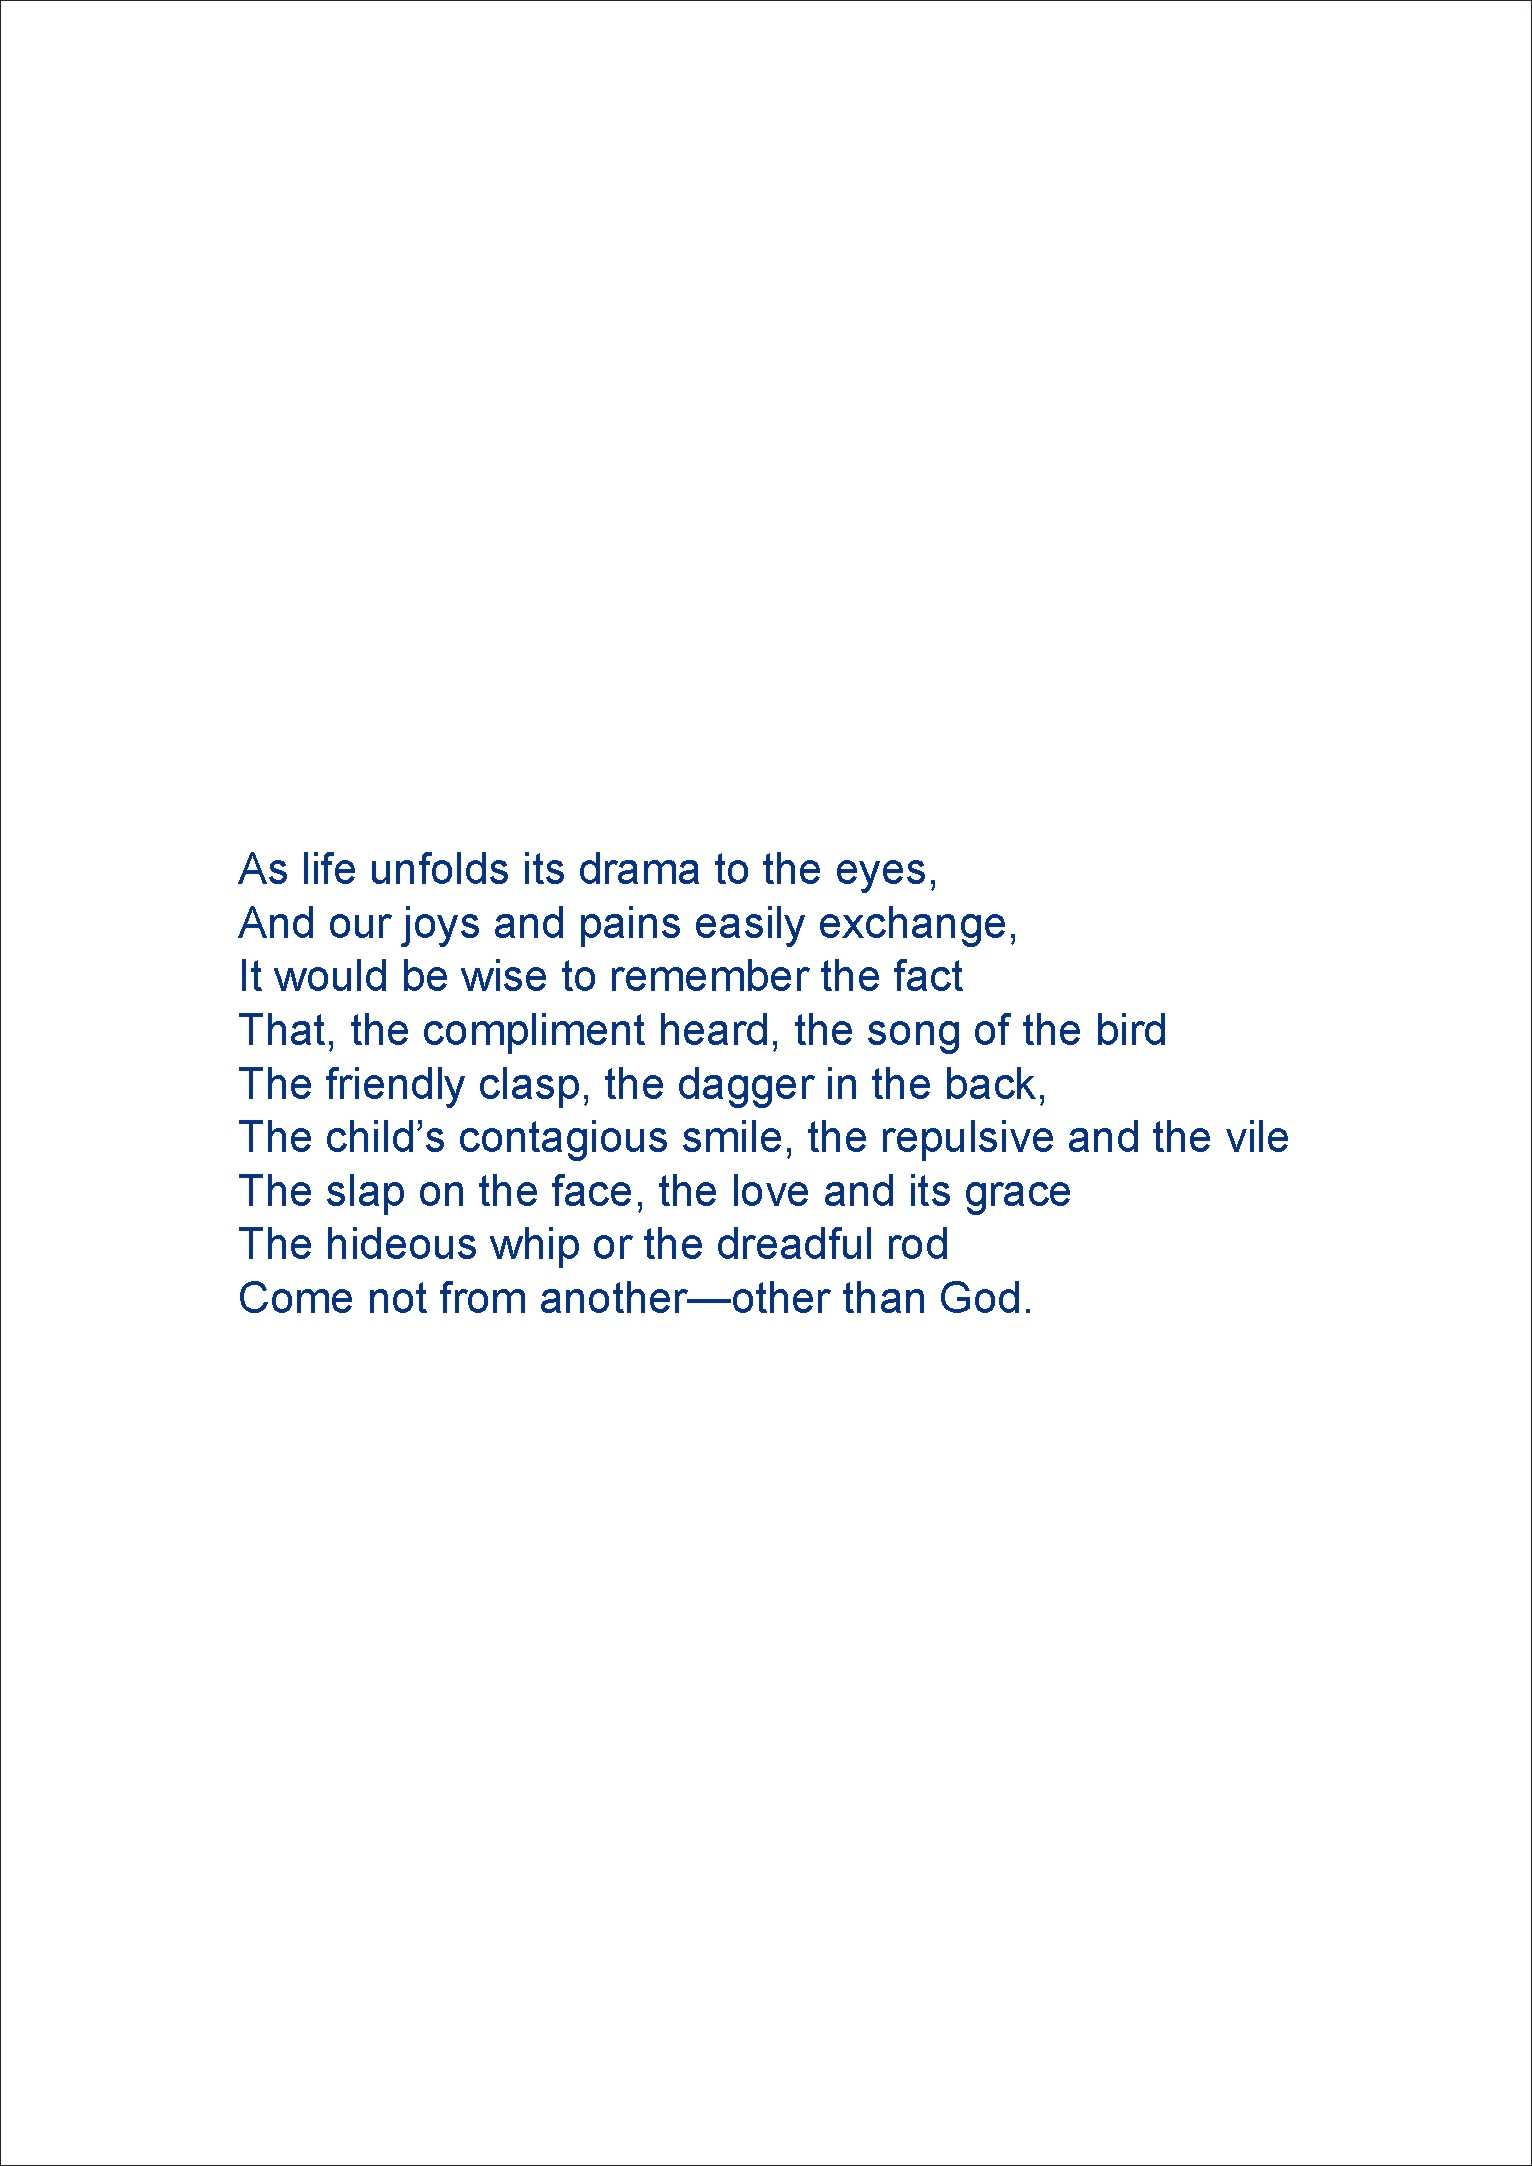
\includegraphics{backCover.jpg}


%% \setlength{\baselineskip}{8.5mm}
%% \
%% \vspace{5cm}

%% \begin{verse}
%% As life unfolds its drama to the eyes,\\
%% And our joys and pains easily exchange,\\
%% It would be wise to remember the fact\\
%% That, the compliment heard, the song of the bird\\
%% The friendly clasp, the dagger in the back,\\
%% The child's contagious smile, the repulsive and~the~vile\\
%% The slap on the face, the love and its grace\\
%% The hideous whip or the dreadful rod\\
%% Come not from another---other than God.
%% \end{verse}


\end{document}
